\section{RQ2: Misinformation and Polarized Toxic Conversations}\label{sec:toxic-polarized-subreddits}
As seen in the previous section, comments are 60\% more toxic under misinformation submissions than authentic news submissions. Furthermore, there appears to be a difference in the political orientation of users that post misinformation and those that comment on it.  Given this difference and the higher toxicity levels present within misinformation submission comments, we now turn to understand if and how these \textit {political differences} drive toxicity within Reddit misinformation submissions. 

\subsection{Experimental Setup}
To fully understand how different levels of \textit{political differences} fuel toxicity and incivility, for this section, we reconstruct the conversational dyads that exist underneath each Reddit submission using the data provided by Pushshift~\cite{baumgartner2020pushshift}. Comments underneath Reddit submissions are similar to conversational threads; if a user responds to a given comment, their reply will appear underneath the comment. For each submission in our dataset, we thus determine using the thread information whether the commenter posted a response directly to another commenter. This then enables us to reconstruct conversational dyads between individual Reddit users. Then, using the approach outlined in Section~\ref{sec:reddit-methods}, we determine the polarization and average toxicity of the users in our conversational dyads. From these calculations, we further label users as conservative/conservative-leaning (positive polarization score) or liberal/liberal-leaning (negative polarization based). Lastly, looking at each of these conversational dyads, we determine if each user's response to each other is toxic/uncivil by utilizing the Perspective API SEVERE\_TOXICITY classifier with a cutoff of 0.8 (as also outlined in Section~\ref{sec:reddit-methods}). For a comparison of how conversations differ between misinformation and authentic news comments, we finally separate out the set of conversational dyads that appear under misinformation and authentic news submissions (for both sets of URLs). 
\begin{figure*}
\begin{subfigure}{.49\textwidth}
  \centering
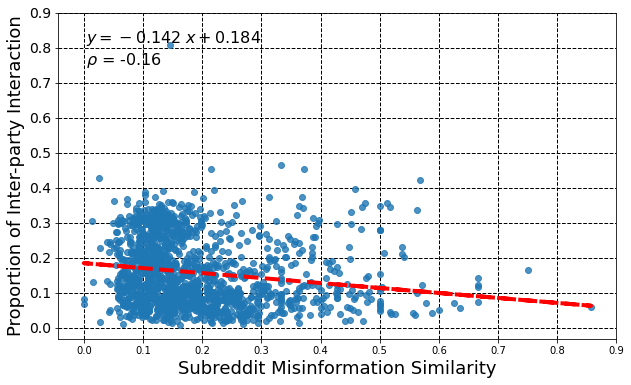
\includegraphics[width=1\linewidth]{figures/subreddit_interparty_interaction.png}

  \label{fig:pagerank-sub2}
\end{subfigure}
\begin{subfigure}{.49\textwidth}
  \centering
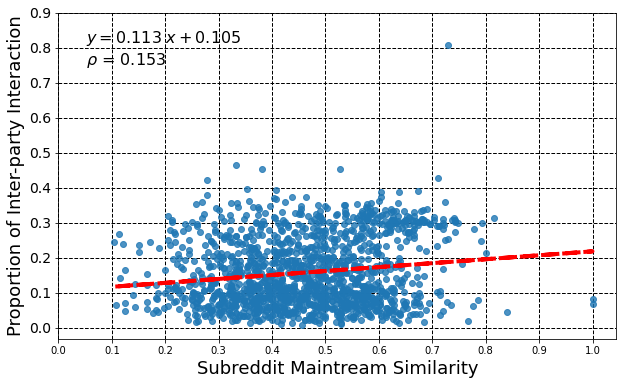
\includegraphics[width=1\linewidth]{figures/subreddit_mainstream_interaction.png}

  \label{fig:pagerank-sub2}
\end{subfigure}
\caption{\textbf{Proportions of inter-party interactions in different subreddits}---As subreddits hyperlink to more \textit{misinfo-oriented} websites, as a percentage, there are fewer and fewer interactions between conservative and liberal users. In contrast, there is a slight correlation between hyperlinking to \textit{mainstream-oriented} websites and more inter-party interactions. }
\label{fig:subreddit-misinformation-mainstream-similarity-interaction}
\end{figure*}




\subsection{Toxic Interactions within Misinformation and Authentic News Environments}
We find high amounts of homophily in interactions across our conversational dyads. Across all our conversational dyads, indeed 81.3\% of interactions are between users of the same political orientation (\textit{i.e} liberal-liberal, conservative-conservative). In contrast, for conversations under mainstream, and misinformation submissions, this increases to 81.7\% and 85.3\% respectively. We thus see slightly more conversational homophily within misinformation conversations than the entire Reddit population at large. Indeed using our set of \textit{misinfo-oriented} and \textit{mainstream-oriented} and looking at subreddits with at least 500 conversational dyads, as seen in Figure~\ref{fig:subreddit-misinformation-mainstream-similarity-interaction}, as website hyperlink to more \textit{misinfo-oriented} websites, conversations on their subreddits become more insular ($\rho =0.160$). In contrast, as subreddits hyperlink to more \textit{mainstream-oriented} websites, there is a slight increase in the amount of inter-party conversations ($\rho =0.153$). We thus see that misinformation is correlated with heightened political homophily within the subreddits, creating more insular communities, while authentic news is associated with a slight increase in political heterophily.

\begin{figure}
\centering
\begin{minipage}[l]{0.4\textwidth}
\centering
\begin{tikzpicture}[very thick]

    % Right square
    \node[fill=gray!20,draw=black, minimum size=1.2cm, inner sep=0pt] (as) {\footnotesize
$0.96\%$};
    \node[draw=black,minimum size=1.2cm, inner sep=0pt, above=-\pgflinewidth of as] (abh) {\footnotesize$0.91\%$};
    \node[draw=black,minimum size=1.2cm, inner sep=0pt, right=-\pgflinewidth of as] (abv) {\footnotesize$0.89\%$};
    \node[fill=gray!20,draw=black, minimum size=1.2cm, inner sep=0pt,  above right=-\pgflinewidth and -\pgflinewidth of as]  {\footnotesize$0.99\%$};
    
    % Side labels
    \node[anchor=east,rotate=90,yshift=0.3cm,xshift=0.7cm] at (as.west) {\scriptsize

Conservative};
    \node[anchor=north,] at (as.south) {\scriptsize
Liberal};
    \node[anchor=east,rotate=90,yshift=0.3cm,xshift=0.5cm] at (abh.west) {\scriptsize
Liberal};
    \node[anchor=north] at (abv.south) {\scriptsize
Conservative};
    
    
    % Square label
    \node[xshift=0.5cm, below=0.5cm of as] {\footnotesize Target};
    
    \node[yshift=1.0cm,xshift=-0.35cm,rotate=90,left=0.5cm of as] {\footnotesize Author};

\end{tikzpicture}
\end{minipage}
\begin{minipage}[c]{0.40\textwidth}
  \caption{\label{fig:interactions}\textbf{Percentage of interactions that are toxic/uncivil for authors and targets of different political leanings.} Across all 46K considered subreddits, there is a slight heterophily for users to reply in a toxic/uncivil manner to members with a tilt towards the opposite political party.}
\end{minipage}
\end{figure}    

Despite the increased political homophily within misinformation filled-subreddits, we observe a reverse trend in terms of toxic/uncivil comments. As seen in Figure~\ref{fig:interactions}, across all considered conversations, we see a slight heterophily for users to reply in a toxic/uncivil manner to users who are not of the same political leaning. We calculate an odds ratio of 1.17 for users to reply in a toxic manner to users of a different political leaning compared with users of the same political leaning. Comparing the set of toxic conversational dyads under misinformation submissions, we see an even higher heterophilic tendency. Compared with the baseline across all conversations, we observe a 25.2\% relative increase in the percentage of liberal to conservative toxic comments and a 12.5\% relative increase in the percentage of conservative to liberal toxic comments. In contrast, for authentic news submissions, we see a 23.2\% relative decrease in liberal to conservative toxic comments and an 18.8\% drop in the percentage of conservative to liberal toxic comments. This appears to indicate that while in misinformation-laced conversations, users are more likely to respond in a toxic manner to users of a different political orientation, users in authentic news-centered conversations are less likely.

To confirm, calculating the odds ratio we get 1.64 for misinformation toxic comments and  0.87 for mainstream toxic comments when comparing the percentages of politically heterophilic toxic comments to politically homophilic comments. Overall we thus find that on average, within misinformation submission comments that users are slightly more likely to respond with a toxic comment to users of different political leaning compared to all submissions on Reddit. This largely explains the higher levels of toxicity observed within misinformation submissions in Section~\ref{sec:toxicity} given the political differences we further observed between misinformation posters and misinformation comments.
 \begin{figure}
    \centering
    \begin{subfigure}{.4\textwidth}
       \centering
\begin{minipage}[c]{\textwidth}
   \centering
\begin{tikzpicture}[very thick]
    % Right square
    \node[fill=red!13,draw=black, minimum size=1.2cm, inner sep=0pt] (as) {\footnotesize$+12.5\%$};
    \node[fill=red!3,draw=black,minimum size=1.2cm, inner sep=0pt, above=-\pgflinewidth of as] (abh) {\footnotesize$+3.3\%$};
    \node[fill=blue!2,draw=black,minimum size=1.2cm, inner sep=0pt, right=-\pgflinewidth of as] (abv) {\footnotesize$-2.2\%$};
    \node[fill=red!25,,draw=black, minimum size=1.2cm, inner sep=0pt,  above right=-\pgflinewidth and -\pgflinewidth of as]  {\footnotesize$+25.2\%$};
    
   % Side labels
    \node[anchor=east,rotate=90,yshift=0.3cm,xshift=0.7cm] at (as.west) {\scriptsize

Conservative};
    \node[anchor=north,] at (as.south) {\scriptsize
Liberal};
    \node[anchor=east,rotate=90,yshift=0.3cm,xshift=0.5cm] at (abh.west) {\scriptsize
Liberal};
    \node[anchor=north] at (abv.south) {\scriptsize
Conservative};
    
    
    % Square label
    \node[xshift=0.5cm, below=0.5cm of as] {\footnotesize Target};
    
    \node[yshift=1.0cm,xshift=-0.35cm,rotate=90,left=0.5cm of as] {\footnotesize Author};


\end{tikzpicture}
\end{minipage}
   \caption{Misinformation Submission comments}
\end{subfigure}
\begin{subfigure}{.4\textwidth}
\begin{minipage}[c]{\textwidth} 
   \centering
\begin{tikzpicture}[very thick]
    % Right square
    \node[fill=blue!19,draw=black, minimum size=1.2cm, inner sep=0pt] (as) {\footnotesize$-18.8\%$};
    \node[fill=blue!9,draw=black,minimum size=1.2cm, inner sep=0pt, above=-\pgflinewidth of as] (abh) {\footnotesize$-8.8\%$};
    \node[fill=blue!8,draw=blue!20,draw=black,minimum size=1.2cm, inner sep=0pt, right=-\pgflinewidth of as] (abv) {\footnotesize$-7.9\%$};
    \node[fill=blue!23,draw=black, minimum size=1.2cm, inner sep=0pt,  above right=-\pgflinewidth and -\pgflinewidth of as]  {\footnotesize$-23.2\%$};
  % Side labels
    \node[anchor=east,rotate=90,yshift=0.3cm,xshift=0.7cm] at (as.west) {\scriptsize

Conservative};
    \node[anchor=north,] at (as.south) {\scriptsize
Liberal};
    \node[anchor=east,rotate=90,yshift=0.3cm,xshift=0.5cm] at (abh.west) {\scriptsize
Liberal};
    \node[anchor=north] at (abv.south) {\scriptsize
Conservative};
    
    
    % Square label
    \node[xshift=0.5cm, below=0.5cm of as] {\footnotesize Target};
    
    \node[yshift=1.0cm,xshift=-0.35cm,rotate=90,left=0.5cm of as] {\footnotesize Author};

\end{tikzpicture}
 \caption{Authentic News Submission comments}
 \end{minipage} 
 \end{subfigure}
   \caption{Percentage increases of interactions that are toxic/uncivil in misinformation submissions for conservative and liberal authors against conservative and liberal targets.}
\end{figure}   

\subsection{Modeling toxic interactions between users commenting under Misinformation Submissions}
In order to confirm the finding that users of different political stripes in misinformation-laced conversations are more likely to reply in a toxic manner to each other, we fit our network data of toxic interactions to an exponential random graph model (ERGM). Exponential Random Graph Models (ERGM) is a form of modeling that predicts connections (toxic interactions) between different nodes (users) in a given network~\cite{hunter2008ergm}. ERGM models assume that connections are determined by a random variable $p^*$ that is dependent on input variables. As in Chen \textit{et al.}~\cite{chen2022misleading} and Peng \textit{et al.}~\cite{peng2016follower}, we utilize this modeling as it does it does not assume that its data input is independent; given that we want to model the interactions of polarization, toxicity, this relaxed restriction is key (we have already seen that they are largely not independent)~\cite{van2019introduction,hunter2008ergm}. Utilizing this framework, we thus model the probability of toxic interactions between a given author and target within misinformation submissions as a function of 1) their percentage of toxic comments, 2) their political polarization, 3) the difference in the author and target's political polarization 4) reciprocity between the author and target (\textit{i.e.} if the author and target both had a toxic comment aimed at each other), and finally 5) the number of subreddits that they share. 
\begin{table}[b]
\centering
\begin{tabular}{lr}
\toprule
   \multicolumn{2}{c}{\large Toxic Misinformation Submission Interactions}          \\
   \toprule
   & Coefficeint \\
      \midrule
      Intercept               &***-8.530 \\               
      \midrule
     Absolute User Polarization       &         -0.464 \\
      \midrule
      User Polarization Differences     & ***-0.782 \\
    \midrule
       User Toxicity &   ***12.396\\
      \midrule
       Reciprocity &  ***4.568\\
      \midrule
       Shared Subreddits &  0.00051\\
\bottomrule
 $\quad\quad\quad\quad ^\ast p<0.05; \;  ^{**} p<0.01; \; ^{***}p<0.001$ \\
\end{tabular}
\caption{As confirmed in our ERGM, differences in political orientation of users is predictive of increased incivility and toxicity. Similarly, the higher each individual user's toxicity norm they are more likely to target other users with toxic comments. }
\label{tbl:ergm}
\end{table}

Fitting our ERGM, we indeed find that as users become more politically distinct from each other, the more likely they are to target each other with uncivil or toxic comments (negative coefficient implies heterophily). As seen in Table~\ref{tbl:ergm}, political polarization by itself does explain toxicity as found by our model; rather differences between users seem to promote toxicity. This largely reinforces are findings from Section~\ref{sec:rq1}. Similarly, as expected, we find that higher levels of user toxicity norms and reciprocity between users are predictive of an increased probability of engaging in toxic interactions. We do not find as users share more subreddits that they are more likely to engage in toxic interactions with each other. 
We thus have seen that not only do misinformation submissions have more insular conversations, with 85.3\% of conversational dyads between users of the same political orientation (compared to 81.3\% of conversations under all Reddit submissions) but also that users become more hostile to users of the opposing political orientation.

\begin{figure*}
\begin{subfigure}{.49\textwidth}
  \centering
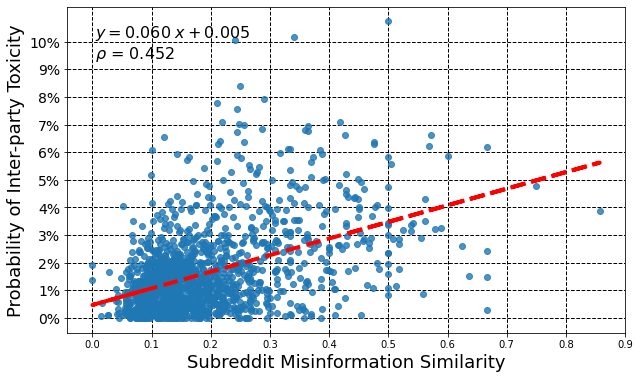
\includegraphics[width=1\linewidth]{figures/subreddit_misinformation_interparty.png}
\label{fig:misinformation-interparty}
\end{subfigure}%s
\begin{subfigure}{.49\textwidth}
  \centering
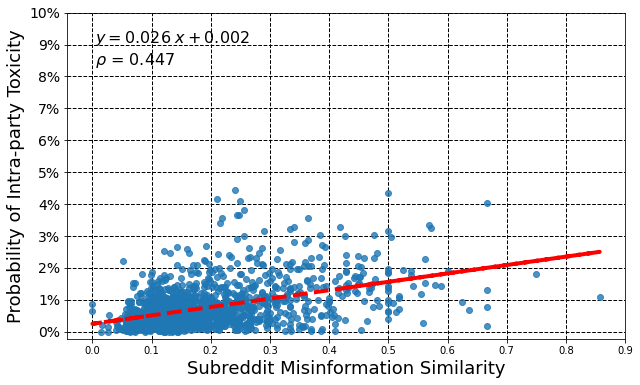
\includegraphics[width=1\linewidth]{figures/subreddit_misinformation_intraparity_toxicity.png}
  \label{fig:misinformation-intrapary}
\end{subfigure}

\caption{\textbf{Subreddit misinformation similarity vs. probability of toxic interactions between users of different and same political orientation}--- While for both inter-political and intra-political interactions, as misinformation similarity in a subreddit increases, the probability of a toxic interaction increases, for inter-political interactions the rate of increase is nearly double. }
\label{fig:subreddit-misinformation-rate-toxictiy-rate}
\end{figure*}


\subsection{Misinformation and increased rates of inter-political toxicity}
Finally, having confirmed that users posting under misinformation submission of different political orientations are more likely to engage in negative interactions with each other, we finally determine if the levels of misinformation within given subreddits as a whole leads to increased heterophilic toxic interactions. Namely as misinformation levels in a subreddit as a whole increase does the probability of negative interactions between users of different political orientations increase. We thus now plot the percentage of misinformation within a given subreddit against the probability of toxic interaction between members of the two political orientations. 


As seen in Figure~\ref{fig:subreddit-misinformation-rate-toxictiy-rate} looking at subreddits with more than 500 conversational dyads, we see that as subreddits have more \textit{misinformation-oriented} hyperlink submissions, the percentage of conversations dyads between users of different political leanings increases. Concretely, subreddit \textit{misinformation similarity} and the probability with which inter-political conversations are toxic have a correlation of $\rho=0.452$. While we similarly see that intra-political toxicity also increases with a similar correlation $\rho=0.447$, we see the rate at which misinformation induces inter-political toxicity is nearly 2.3 times that of intra-political toxicity (0.060 slope vs 0.026 slope). This reflects the fact that \textit{misinformation oriented} submissions are on the whole more toxic but that they increase politically heterophilic toxicity more than politically homophilic toxicity. 
\begin{figure*}
\begin{subfigure}{.49\textwidth}
  \centering
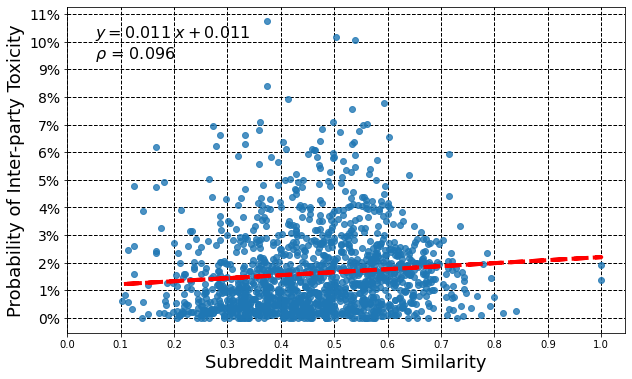
\includegraphics[width=1\linewidth]{figures/subreddit_mainstream_toxicity_interparty.png}
\label{fig:misinformation-interparty}
\end{subfigure}%s
\begin{subfigure}{.49\textwidth}
  \centering
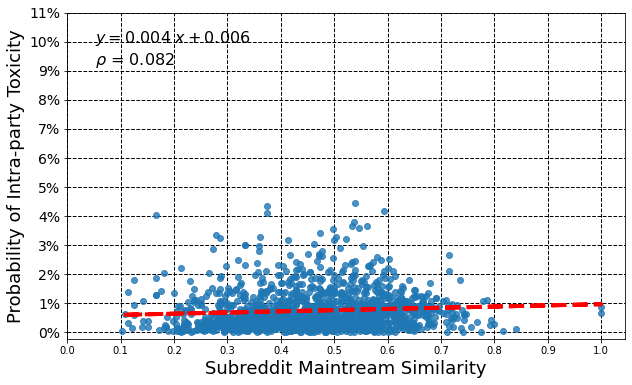
\includegraphics[width=1\linewidth]{figures/mainstream_intra_party_toxic.png}
  \label{fig:misinformation-intrapary}
\end{subfigure}

\caption{\textbf{Subreddit misinformation similarity vs. probability of toxic interactions between users of different and same political orientation}--- For both inter-political and intra-political interactions, as mainstream similarity in a subreddit increases the probability of inter- and intra-political toxicity is largely flat.}
\label{fig:subreddit-mainstram-rate-toxictiy-rate}
\end{figure*}

Again comparing against subreddit mainstream similarity, we do not see a similar relationship. As seen in Figure~\ref{fig:subreddit-mainstram-rate-toxictiy-rate}, the relationship between inter-political and intra-political toxicity rates and similarity to mainstream sources is largely flat. 


\subsection{Summary} Misinformation, we find, not only promotes higher levels of toxicity in general but also appears to drive inter-political incivility. Fitting an ERGM to our misinformation toxic dyads, we indeed find that political differences (along with reciprocity and each user's toxicity) are a driving force behind the formation of a toxic conversational thread. Finally, examining how different levels of misinformation promote toxicity among users, we find that across our considered subreddits, misinformation drives inter-political incivility at 2.3 times the rate of intra-political toxicity. 





















 





%We now seek gain an understanding of whether Reddit subreddits where the misinformation URLs  were posted or the users commenting in the submissions themselves were driving the toxicity within the misinformation submissions. As seen in Figure~\ref{}, misinformation subreddits in both 



    






























